\ChapterImageStar[cap:revisionLiteratura]{Revisión sistemática de la literatura}{./images/fondo.png}\label{cap:revisionLiteratura}

\mbox{}\\
\section{Construcción de la bitácora}

En busca de una base teórica sólida para seleccionar un nuevo universo HTCondor y con el objetivo de tomar decisiones informadas, se llevó a cabo una revisión exhaustiva de la literatura existente sobre el tema. Este proceso se desarrolló en varias etapas:


\subsection{Planeación}

Esta etapa consistió en establecer el propósito general que se buscaba alcanzar con el \SMS (\textit{Systematic Mapping Study}).
A su vez, definió aspectos como objetivos ver cuadro ~\ref{tab:metas}, preguntas de investigación ver cuadro~\ref{tab:preguntas} y métricas ver cuadro~\ref{tab:metricas}. Para ello, se siguió el modelo
Objetivo-Pregunta-Métrica (\textit{goal-question-metric}, gqm). A continuación, se definen los objetivos del \SMS\ aplicado
a los universos de HTCondor en el cuadro.

\subsubsection{Definición de metas para el \SMS}

% Tabla METAS DEL SMS
\begin{table}[H]
	\centering
	\renewcommand{\arraystretch}{1.2} % Espaciado reducido
	\footnotesize % Texto más pequeño
	\begin{tabular}{|p{1.5cm}|p{12.5cm}|}  % Total: 14cm
		\hline
		\textbf{Meta} & \textbf{Descripción}                                                                                                                                                                                                                                                                                                                                         \\ \hline
		G1            & Clasificar trabajos relacionados con los universos de HTCondor según su aplicación e impacto en los dominios de computación distribuida y paralela, HTC, desarrollo de Software, virtualización y microservicios, redes de computadoras, infraestructura computacional, inteligencia artificial, análisis de datos y pensamiento computacional, entre otros. \\ \hline
		G2            & Identificar y categorizar trabajos vinculados con los universos de HTCondor como herramienta para fortalecer funciones esenciales universitarias como: investigación, docencia, extensión e industria.                                                                                                                                                       \\ \hline
	\end{tabular}
	\caption{Definición de metas del SMS}
	\label{tab:metas}
\end{table}

\subsubsection{Definición de preguntas de investigación}
%TABLA GOAL VS Preguntas 
\begin{table}[H]
	\centering
	\renewcommand{\arraystretch}{1.2} % Espaciado reducido
	\scriptsize % Texto más pequeño
	\begin{tabular}{|p{0.7cm}|p{1.3cm}|p{5.5cm}|p{6cm}|} % Total: 14cm
		\hline
		\textbf{Meta}                                                                                                                                                                                                                                                                                                                                    & \textbf{Pregunta} & \textbf{Descripción} & \textbf{Motivación}       \\ \hline

		G1                                                                                                                                                                                                                                                                                                                                               & Q1                &
		\textit{¿Qué trabajos relacionados con los universos de HTCondor tienen impacto en los dominios de computación distribuida y paralela, HTC, desarrollo de Software, virtualización y microservicios, redes de computadoras, infraestructura computacional, inteligencia artificial, análisis de datos y pensamiento computacional, entre otros?} &
		Sobre los universos de HTCondor que tienen impacto en los dominios de computación distribuida y paralela, HTC, desarrollo de Software, virtualización y microservicios, redes de computadoras, infraestructura computacional, inteligencia artificial, análisis de datos, pensamiento computacional: 1 - Reconocer cómo están estructurados. 2 - Identificar sus aplicaciones. 3 - Determinar su motivación contextual. \\ \hline

		G2                                                                                                                                                                                                                                                                                                                                               & Q2                &
		\textit{¿Qué trabajos vinculados con los universos de HTCondor potencian las funciones esenciales universitarias como investigación, docencia, extensión e industria?}                                                                                                                                                                           &
		Sobre los universos de HTCondor que potencian las funciones sustantivas universitarias como investigación, docencia, extensión e industria: 1 - Reconocer cómo están estructurados. 2 - Identificar sus aplicaciones. 3 - Determinar su motivación contextual.                                                                                                                                                          \\ \hline
	\end{tabular}
	\caption{Definición de preguntas de investigación del SMS}
	\label{tab:preguntas}
\end{table}

\subsubsection{Definición de métricas}
%Tabla METRICAS
\begin{table}[H]
	\centering
	\renewcommand{\arraystretch}{1.2} % Menor espaciado entre filas
	\footnotesize % Texto más pequeño
	\begin{tabular}{|c|p{13cm}|} % Total: 14cm
		\hline
		\textbf{Métrica} & \textbf{Descripción}                                                                                                                                                                                                                                                                                                                                                                                                                                                                                           \\ \hline
		M1               & Cantidad de trabajos relacionados con los Universos de HTCondor vinculados con los dominios de: Computación distribuida y paralela, HTC, Desarrollo de software, Tecnologías de virtualización y microservicios, Redes de computadores, Infraestructura computacional, Inteligencia artificial, Análisis de datos, Pensamiento computacional, entre otros. Y que además sean usados como herramienta para fortalecer funciones esenciales universitarias como: Investigación, Docencia, Extensión e Industria. \\ \hline
		M2               & Popularidad de cada Universo en los trabajos seleccionados.                                                                                                                                                                                                                                                                                                                                                                                                                                                    \\ \hline
		M3               & Porcentaje de trabajos seleccionados en la fase final respecto de la cantidad de trabajos iniciales.                                                                                                                                                                                                                                                                                                                                                                                                           \\ \hline
		M4               & Porcentaje de trabajos aportados por cada base de datos en el mapeo que se está desarrollando.                                                                                                                                                                                                                                                                                                                                                                                                                 \\ \hline
	\end{tabular}
	\caption{Definición de métricas del SMS}
	\label{tab:metricas}
\end{table}

\section{Búsqueda de estudios}

Esta etapa comprendió las siguientes secciones:
\begin{enumerate}
	\item Estrategia de búsqueda, ya sea independiente o combinada;
	\item Identificación general de estudios;
	\item Revisión de estudios; y finalmente,
	\item Selección de estudios para incluir en el SMS.\@
\end{enumerate}

\subsection{Estrategia de búsqueda}

Este trabajo combinó las estrategias de búsqueda en bases de datos y búsqueda en bola de nieve.

\subsection{Búsqueda en bases de datos}\label{subsec:busquedaBasesDatos}
Se seleccionaron las siguientes bases de datos para este propósito: ACM, IEEE Xplore, Springer, Taylor \& Francis y Science Direct.

\subsubsection{Identificación de estudios mediante búsqueda en bases de datos}\label{subsubsec:identificacionEstudios}
En esta etapa del proceso fue necesario establecer las palabras clave que serían útiles en las cadenas de búsqueda para cada una de las bases de datos seleccionadas.
Los términos consideran los elementos identificados en la etapa de planificación, para lo cual también se utilizó el modelo PICOC ( \textit{Population}, \textit{Intervention}, \textit{Comparator}, \textit{Outcome}, and \textit{Context} ) como guía metodológica.

% TABLA modelo PICOC: Población - Intervención - Comparación  - Salida - Contexto
\begin{table}[H]
	\centering
	\renewcommand{\arraystretch}{1.2} % Espaciado reducido
	\footnotesize % Texto más pequeño
	\begin{tabular}{|c|p{12cm}|} % Total: 14cm
		\hline
		\textbf{Componente} & \textbf{Descripción}                                                                                                                                                                                                                                                                                                                                                                                                                                                                             \\ \hline

		Población           & Trabajos relacionados con los universos de HTCondor según su aplicación e impacto en los dominios de computación distribuida y paralela, HTC, desarrollo de Software, virtualización y microservicios, redes de computadoras, infraestructura computacional, inteligencia artificial, análisis de datos, pensamiento computacional, entre otros. Que potencian las funciones sustantivas universitarias de investigación, docencia y extensión.                                                  \\ \hline

		Intervención        & Identificación y clasificación de un conjunto de trabajos relacionados con los universos de HTCondor según su aplicación e impacto en los dominios de computación distribuida y paralela, HTC, desarrollo de Software, virtualización y microservicios, redes de computadoras, infraestructura computacional, inteligencia artificial, análisis de datos, pensamiento computacional, entre otros. Que potencian las funciones sustantivas universitarias de investigación, docencia y extensión. \\ \hline

		Comparación         &
		\textbf{1.} Casos de proyecto documentados.
		\textbf{2.} Cumplimiento de criterios de inclusión y exclusión.
		\textbf{3.} Aparición en bases de datos seleccionadas.                                                                                                                                                                                                                                                                                                                                                                                                                                                                 \\ \hline
		Salida              & Taxonomía que organiza los trabajos relacionados con los universos de HTCondor según su aplicación e impacto en los dominios de computación distribuida y paralela, HTC, desarrollo de Software, virtualización y microservicios, redes de computadoras, infraestructura computacional, inteligencia artificial, análisis de datos, pensamiento computacional, entre otros. Que potencian las funciones sustantivas universitarias de investigación, docencia y extensión.                       \\ \hline
		Contexto            & Universos HTCondor en dominios de computación distribuida y paralela, HTC, desarrollo de Software, virtualización y microservicios, redes de computadoras, infraestructura computacional, inteligencia artificial, análisis de datos, pensamiento computacional, entre otros. Que potencian las funciones sustantivas universitarias de investigación, docencia y extensión.                                                                                                                     \\ \hline
	\end{tabular}
	\caption{Modelo PICOC}
\end{table}


%# TABLA Palabras clave indentificadas usando el modelo PICOC.
\begin{table}[H]
	\centering
	\scriptsize
	\setlength{\tabcolsep}{2pt}
	\renewcommand{\arraystretch}{1.2}
	\fontsize{6}{10}\selectfont
	\begin{tabular}{|p{2.8cm}|p{2.8cm}|p{2.0cm}|p{2.8cm}|p{2.8cm}|} % Total: 14cm
		\hline
		\textbf{Población}            & \textbf{Intervención} & \textbf{Criterios de aceptación} & \textbf{Salidas} & \textbf{Contexto} \\
		\hline
		- Trabajos relacionados \newline
		- Universos \newline
		- HTCondor \newline
		- Computación distribuida y paralela \newline
		- HTC \newline
		- Desarrollo de Software \newline
		- Virtualización y microservicios \newline
		- Redes de computadoras \newline
		- Infraestructura computacional \newline
		- Inteligencia artificial \newline
		- Análisis de datos \newline
		- Pensamiento computacional \newline
		- Investigación \newline
		- Docencia \newline
		- Extensión                   &
		- Identificación \newline
		- Clasificación \newline
		- Universos \newline
		- HTCondor \newline
		- Computación distribuida y paralela \newline
		- HTC \newline
		- Desarrollo de Software \newline
		- Virtualización y microservicios \newline
		- Redes de computadoras \newline
		- Infraestructura computacional \newline
		- Inteligencia artificial \newline
		- Análisis de datos \newline
		- Pensamiento computacional \newline
		- Investigación \newline
		- Docencia \newline
		- Extensión                   &
		- Casos de estudio culminados &
		- Taxonomía \newline
		- Universos \newline
		- HTCondor \newline
		- Computación distribuida y paralela \newline
		- HTC \newline
		- Desarrollo de Software \newline
		- Virtualización y microservicios \newline
		- Redes de computadoras \newline
		- Infraestructura computacional \newline
		- Inteligencia artificial \newline
		- Análisis de datos \newline
		- Pensamiento computacional \newline
		- Investigación \newline
		- Docencia \newline
		- Extensión                   &
		- Universos \newline
		- HTCondor \newline
		- Computación distribuida y paralela \newline
		- HTC \newline
		- Desarrollo de Software \newline
		- Virtualización y microservicios \newline
		- Redes de computadoras \newline
		- Infraestructura computacional \newline
		- Inteligencia artificial \newline
		- Análisis de datos \newline
		- Pensamiento computacional \newline
		- Investigación \newline
		- Docencia \newline
		- Extensión                                                                                                                     \\
		\hline
	\end{tabular}
	\caption{Palabras clave identificadas usando el modelo PICOC}
	\label{table:keywords-picoc}
\end{table}

Las palabras clave identificadas en el cuadro~\ref{table:keywords-picoc} se complementaron con sinónimos y términos relacionados, los cuales se presentan en el cuadro~\ref{tab:keywords}. Estas keywords se utilizaron para construir las cadenas de búsqueda en cada base de datos.


%# TABLA Keywoords para las cadenas de búsqueda,
\begin{table}[H]
	\centering
	\scriptsize
	\setlength{\tabcolsep}{4pt}
	\begin{tabular}{|c|p{11.5cm}|} % Total: 14cm
		\hline
		\textbf{Palabras clave} & \textbf{Sinónimos}                                                             \\
		\hline
		HTCondor                & High Throughput Condor, Distributed Computing Framework, Condor                \\
		\hline
		HTC                     & HPC, High Throughput Computing, High Performance Computing                     \\
		\hline
		Universe                & Execution Environment, Runtime Environment, Cluster                            \\
		\hline
		Project                 & Work, Implementation, Implement, Deployment, Development, Program, Plan, Study \\
		\hline
		Research                & Teaching, Extension, Outreach, Industry                                        \\
		\hline
	\end{tabular}
	\caption{Palabras clave para la búsqueda en base de datos}
	\label{tab:keywords}
\end{table}



\noindent
Con el objetivo de filtrar los resultados y enfocarse en estudios relevantes, se definieron criterios de inclusión y exclusión, los cuales se presentan en el cuadro~\ref{table:criterios-inclusion-exclusion}. Estos criterios ayudaron a seleccionar artículos que se alinean con los objetivos del \SMS y a descartar aquellos que no aportan valor al análisis\dots

% TABLA Criterios de inclusión y exclusión
\begin{table}[H]
	\centering
	\caption{Criterios de inclusión y exclusión}
	\begin{tabular}{|p{3cm}|p{5cm}|p{6cm}|}
		\hline
		\textbf{Categoría}  & \textbf{Inclusión}         & \textbf{Exclusión}                                                                                                          \\
		\hline
		Tipo de publicación & Artículos de investigación & Tesis, capítulos de libros, libros, revistas, conferencias, y todo lo demás que no esté en el tipo de publicación inclusiva \\
		\hline
		Período             & Desde 2020 hasta 2024      & -                                                                                                                           \\
		\hline
		Idioma              & Inglés                     & -                                                                                                                           \\
		\hline
	\end{tabular}
	\label{table:criterios-inclusion-exclusion}
\end{table}



%##################
%##################
%##################
%##################
%##################




\subsubsection{Búsqueda en bases de datos}\label{par:busquedaBasesDatos}
\noindent
Las cadenas de búsqueda específicas para cada base de datos se encuentran en la sección~\ref{sec:cadenas-busqueda} del apéndice.

\subsubsection{Métricas de la búsqueda sin criterios de inclusión/exclusión}\label{subsubsec:resumenBusqueda}
\noindent
La Tabla~\ref{table:bases-sin-exclusion} presenta el número de publicaciones identificadas en las principales bases de datos consultadas durante la revisión inicial de literatura, antes de aplicar los criterios de inclusión y exclusión. En total se recuperaron 847 registros, distribuidos de la siguiente manera: ACM (518), IEEE (0), Springer (209), Science Direct (120) y Taylor \& Francis (0). Estos resultados se evidencian en el apéndice~\ref{sec:busqueda-sin-criterios}.

% TABLA Resultados de busqueda sin exclusión
\begin{table}[H]
	\centering
	\caption{Resultados de las cadenas de búsqueda}
	\label{table:bases-sin-exclusion}
	\begin{tabular}{|p{4.5cm}|c|c|c|c|c|c|}
		\hline
		\textbf{Criterios}                               & \textbf{ACM} & \textbf{IEEE} & \textbf{ScienceDirect} & \textbf{Springer} & \textbf{Taylor\&Francis} & \textbf{Total} \\
		\hline
		Cadena de búsqueda con palabras clave únicamente & 518          & 0             & 120                    & 209               & 0                        & 847            \\
		\hline
		Contribución porcentual                          & 61.16\%      & 0\%           & 14.17\%                & 24.68\%           & 0\%                      & 100\%          \\
		\hline
	\end{tabular}
\end{table}



\subsubsection{Métricas de la búsqueda con criterios de inclusión/exclusión}\label{subsec:resumenBusquedaCriterios}
\noindent
Esta búsqueda se realizó considerando los criterios de exclusión e inclusión definidos previamente. Las cadenas de búsqueda son exactamente iguales que antes, este punto se diferencia por la aplicación de filtros. Para ver las capturas de pantalla veáse el apéndice~\ref{sec:busqueda-con-criterios}.
La Tabla~\ref{table:bases-con-exclusion} muestra los resultados obtenidos tras aplicar los criterios de inclusión y exclusión previamente definidos. A diferencia de la búsqueda inicial, en esta fase se utilizaron filtros específicos que redujeron significativamente la cantidad de publicaciones relevantes. En total se identificaron 976 documentos, distribuidos en las bases de datos de la siguiente manera: ACM (48), IEEE (134), Springer (592), Science Direct (46) y Taylor \& Francis (156).

% TABLA Bases de datos con inclusión
\begin{table}[H]
	\centering
	\caption{Resultados de las cadenas de búsqueda con criterios de exclusión}
	\label{table:bases-con-exclusion}
	\begin{tabular}{|p{4.5cm}|c|c|c|c|c|c|}
		\hline
		\textbf{Criterios}                               & \textbf{ACM} & \textbf{IEEE} & \textbf{ScienceDirect} & \textbf{Springer} & \textbf{Taylor \& Francis} & \textbf{Total} \\
		\hline
		Cadena de búsqueda con palabras clave únicamente & 315          & 0             & 101                    & 63                & 0                          & 479            \\
		\hline
		Contribución porcentual                          & 65.76\%      & 0\%           & 21.09\%                & 13.15\%           & 0\%                        & 100\%          \\
		\hline
	\end{tabular}
\end{table}





\begin{table}[H]
\centering
\scriptsize
\setlength{\tabcolsep}{4pt}
\renewcommand{\arraystretch}{1.1}
\begin{tabular}{|l|c|c|c|c|c|c|}
\hline
\textbf{Bases de datos} & \textbf{ACM} & \textbf{IEEE} & \textbf{Springer} & \textbf{Science Direct} & \textbf{Taylor \& Francis} & \textbf{Total} \\
\hline
Sin aplicar criterios & 189 & 426 & 4562 & 353 & 1000 & 6530 \\
\hline
Con criterios aplicados & 48 & 134 & 592 & 46 & 156 & 976 \\
\hline
\end{tabular}
\caption{Resumen de la búsqueda en bases de datos con criterios de inclusión/exclusión}\label{tab:resumen-busqueda}
\end{table}
\begin{figure}[H]
    \centering
    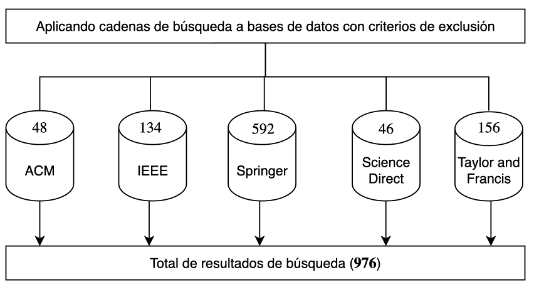
\includegraphics[scale=0.9] {tablas-images/cp2/bases-con-criterio.png}
    \caption{Resumen de la búsqueda en bases de datos con criterios de inclusión/exclusión}\label{fig:tabla-resumen-busqueda-con-criterio}
\end{figure}

\section{Eliminación de duplicados}\label{sec:eliminacionDuplicados}
\noindent
La eliminación de duplicados se realizó haciendo uso de la herramienta de gestión de referencias Mendeley. Luego de obtener los artículos se agregaron a Mendeley y esta herramienta se encargó de eliminar duplicados. En este punto se eliminaron 274 artículos duplicados.

\section{Priorización de estudios}\label{sec:priorizacionEstudios}
\noindent
Luego de la selección inicial de los artículos, se procedió a revisar el \textit{title}, \textit{abstract} y \textit{keywords} de cada uno. Como resultado de esta revisión, se generaron métricas de calidad para cada artículo, con el fin de priorizar aquellos más relevantes para la investigación. Las métricas utilizadas fueron las siguientes:

\begin{itemize}
	\item \textbf{SCI} \textit{(Science Citation Index)}
	\item \textbf{CVI} \textit{(Core Value Index)}
	\item \textbf{IRRQ} \textit{(Index Relation Research Question)}
\end{itemize}
\noindent
Este proceso inició con un total de 771 artículos, los cuales fueron evaluados según su alineamiento con los objetivos de la investigación. La evaluación temática permitió identificar un total de 110 artículos con una relación directa con el enfoque planteado.

\section{Estrategia de búsqueda usando bola de nieve}\label{sec:bolaDeNieve}
\noindent
En esta etapa, se seleccionó el primer cuartil según el índice SCI, lo que resultó en un total de 24 artículos. Adicionalmente, se incluyó un artículo por criterio de inclusión directa, estableciendo así una línea base de 25 artículos.
Partiendo de esta base, se aplicó la estrategia de bola de nieve en dos direcciones: hacia adelante y hacia atrás. Como resultado, se obtuvieron 87 artículos aplicando la técnica hacia atrás y 495 artículos aplicando la técnica hacia adelante.
Esto definió un nuevo conjunto de artículos para un proceso de selección adicional (\textit{screening}). En esta fase, se eliminaron 14 duplicados y 452 artículos fueron descartados por no aportar valor a la investigación.
Finalmente, se obtuvo un total de 116 artículos mediante esta estrategia de búsqueda.

\section{Diagrama de búsqueda}\label{sec:diagramaBusqueda}

\subsection{Usando cadenas de búsqueda}
\noindent
En el diagrama~\ref{tab:tabla-diagrama-cadena-busqueda} se puede apreciar la estrategia de búsqueda de artículos por medio de base de datos, aplicando las cadenas de búsqueda, se consolidaron los resultados de distintas bases de datos para obtener un total de 6530 resultados, posteriormente y aplicando criterios de exclusión se redujo esta cantidad a menos de 1000 resultados. Adicional a los criterios de exclusión, también se hizo eliminación de artículos duplicados, 205 por parte del ~\textit{Reference Manager}, y 69 por parte del ~\textit{SMS-Builder} para un total de 274 artículos removidos. Finalmente, se realiza la etapa de screening, donde se leen las secciones claves de los artículos, como ~\textit{abstract}, ~\textit{keywords} e introducción, a través de esto se pudo descargar 593 artículos que no eran pertinentes para el estudio.
\begin{table}[H]
    \centering
    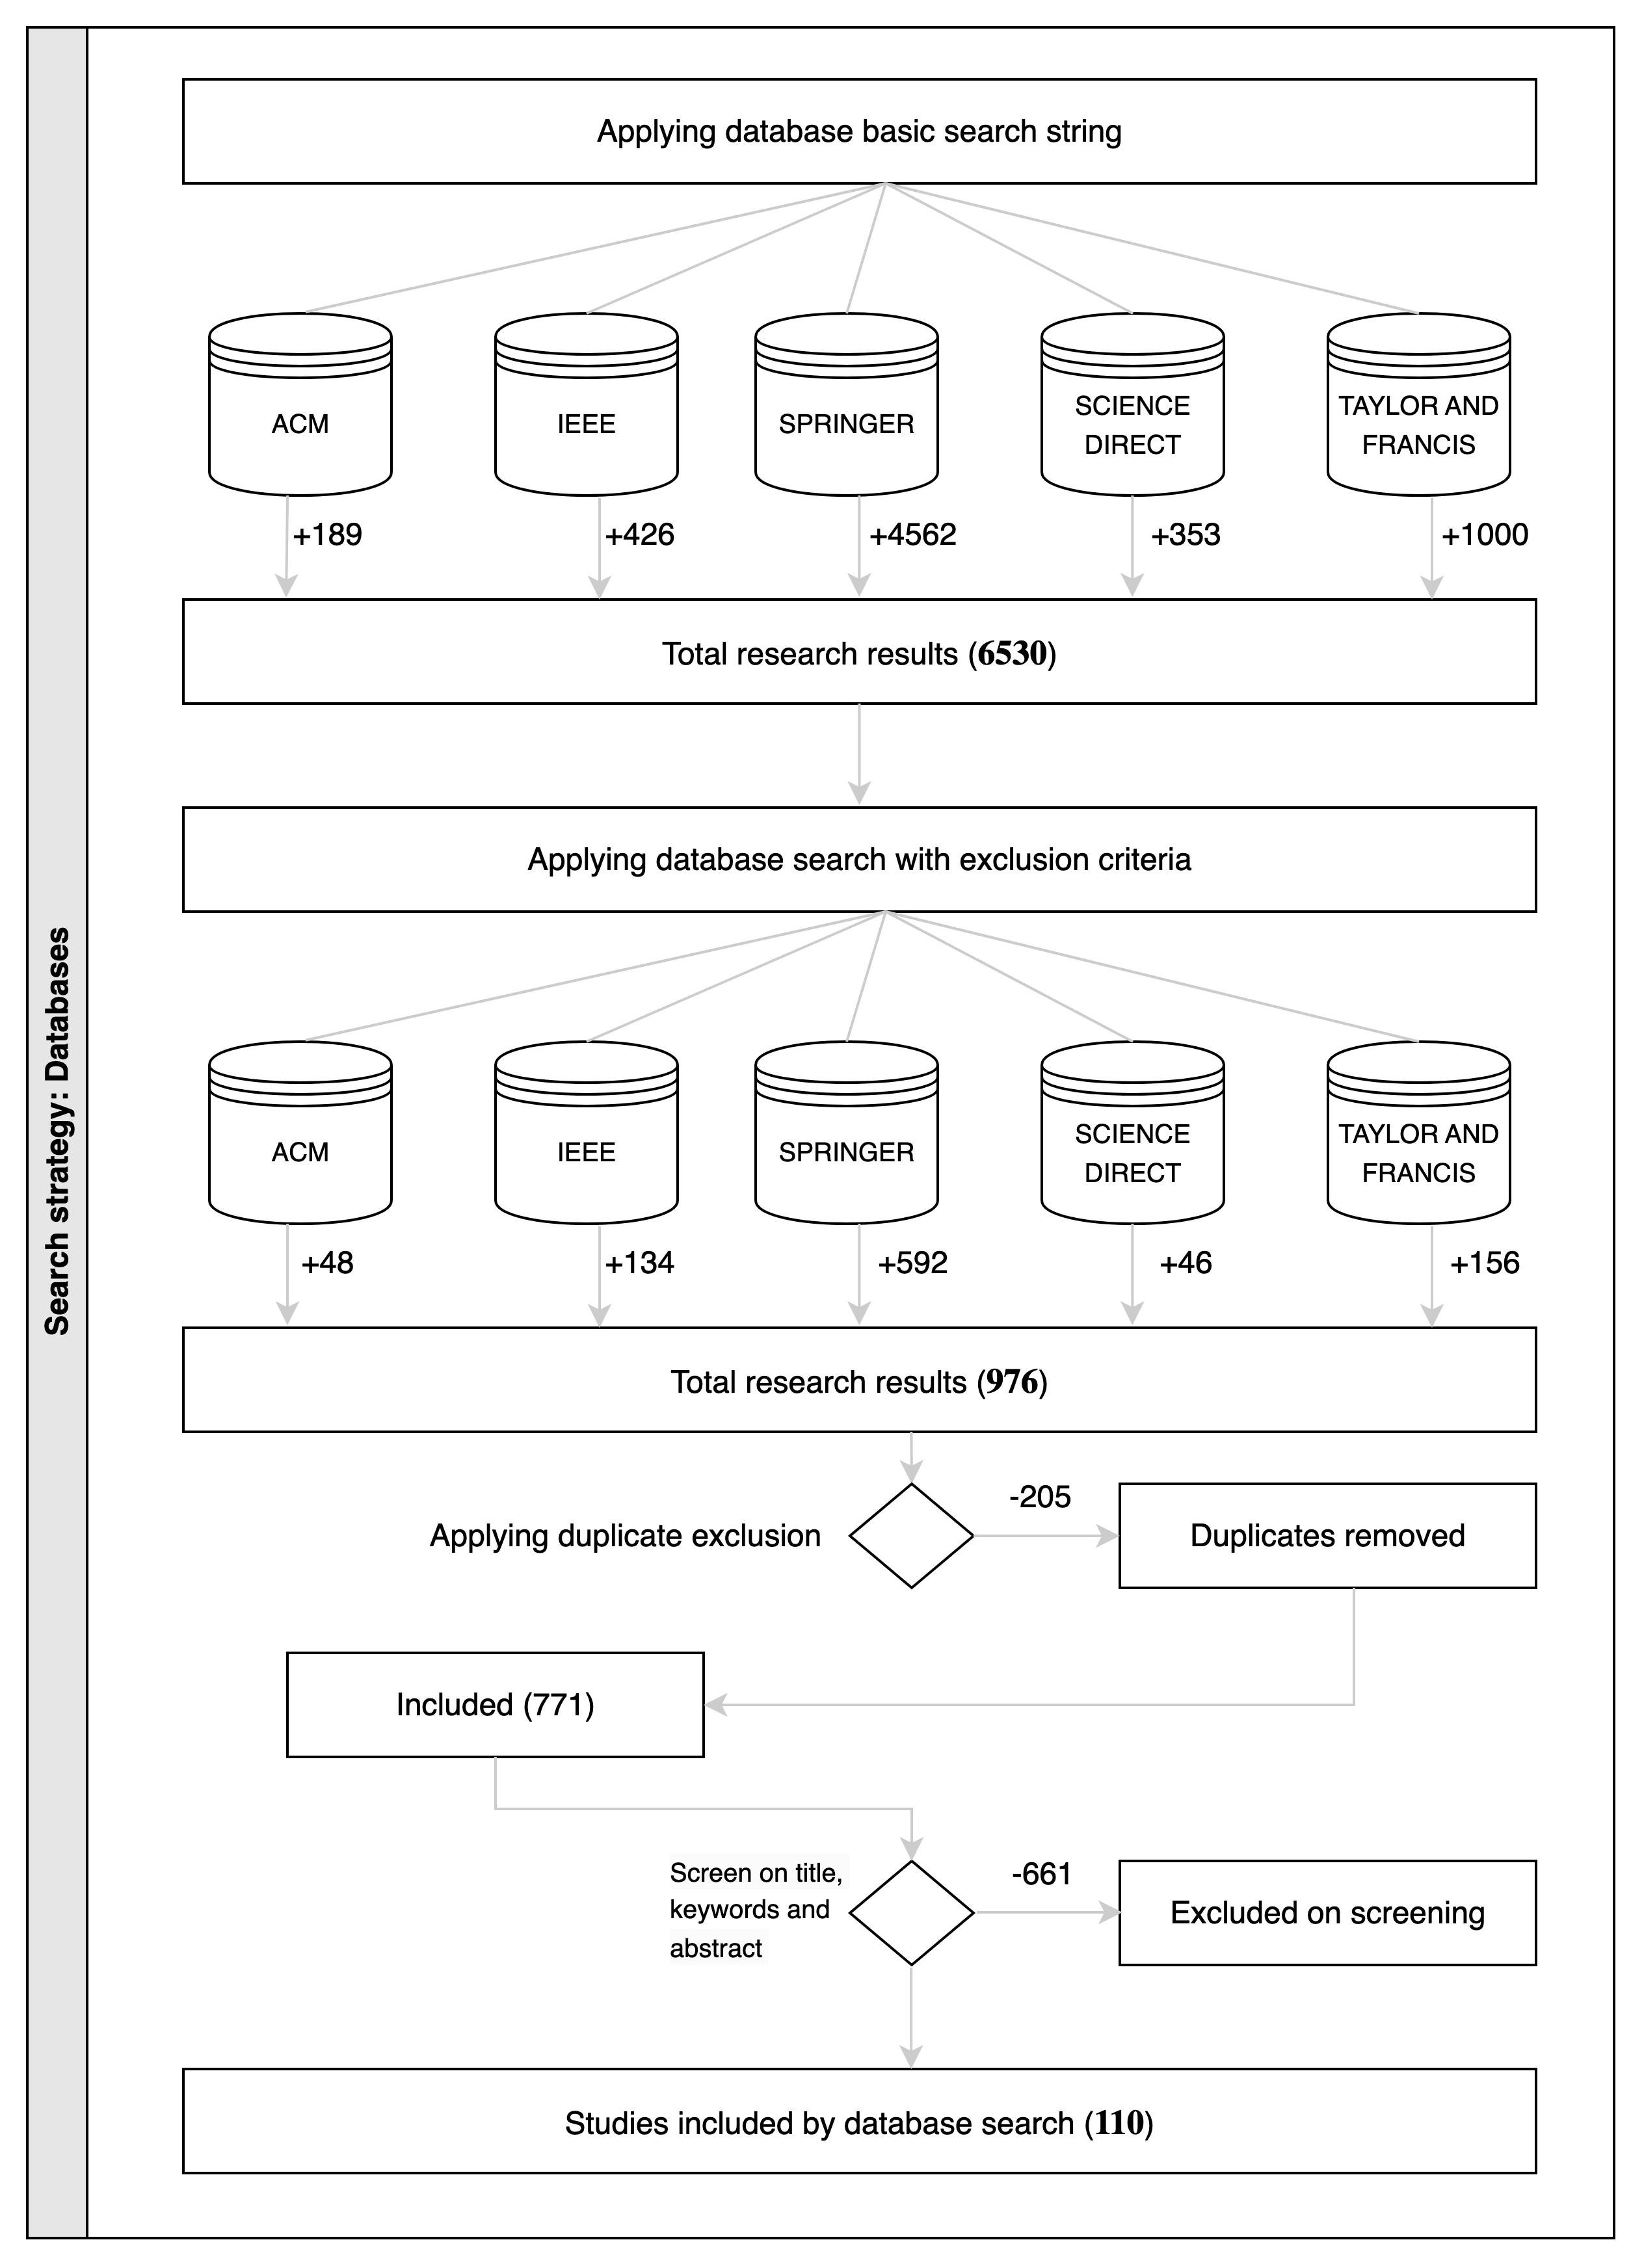
\includegraphics[scale=0.13]{tablas-images/cp2/diagrama-cadena-busqueda.png}
    \caption{Diagrama de la cadena de búsqueda}\label{tab:tabla-diagrama-cadena-busqueda}
\end{table}\label{img:busqueda-bd}

\subsection{Usando bola de nieve}
\noindent
Como segunda estrategia de búsqueda dentro del SMS, se aplicó la técnica de ~\textit{Snowball}, la cual consiste en extraer artículos adicionales a partir de las referencias citadas en los estudios obtenidos en la estrategia anterior y de los estudios que citan a estos. De los 110 estudios del paso anterior, se seleccionan aquellos que tenían un SCI más alto (primer cuartil) y se agrega uno por inclusión directa, con esto se obtiene un total de 25 artículos de línea base. Aplicando la técnica hacia adelante (artículos referenciados) se obtienen 87 nuevos estudios y la misma hacia atrás (artículos que referencian el artículo base) se obtienen 495, para un total de 582. Finalmente, se filtraron duplicados para iniciar la revisión del \textit{screening}. Como resultado 116 artículos fueron incluidos por bola de nieve. Todo este proceso se puede apreciar en la gráfica~\ref{tab:tabla-diagrama-bola-nieve-busqueda}.
\begin{table}[H]
    \centering
    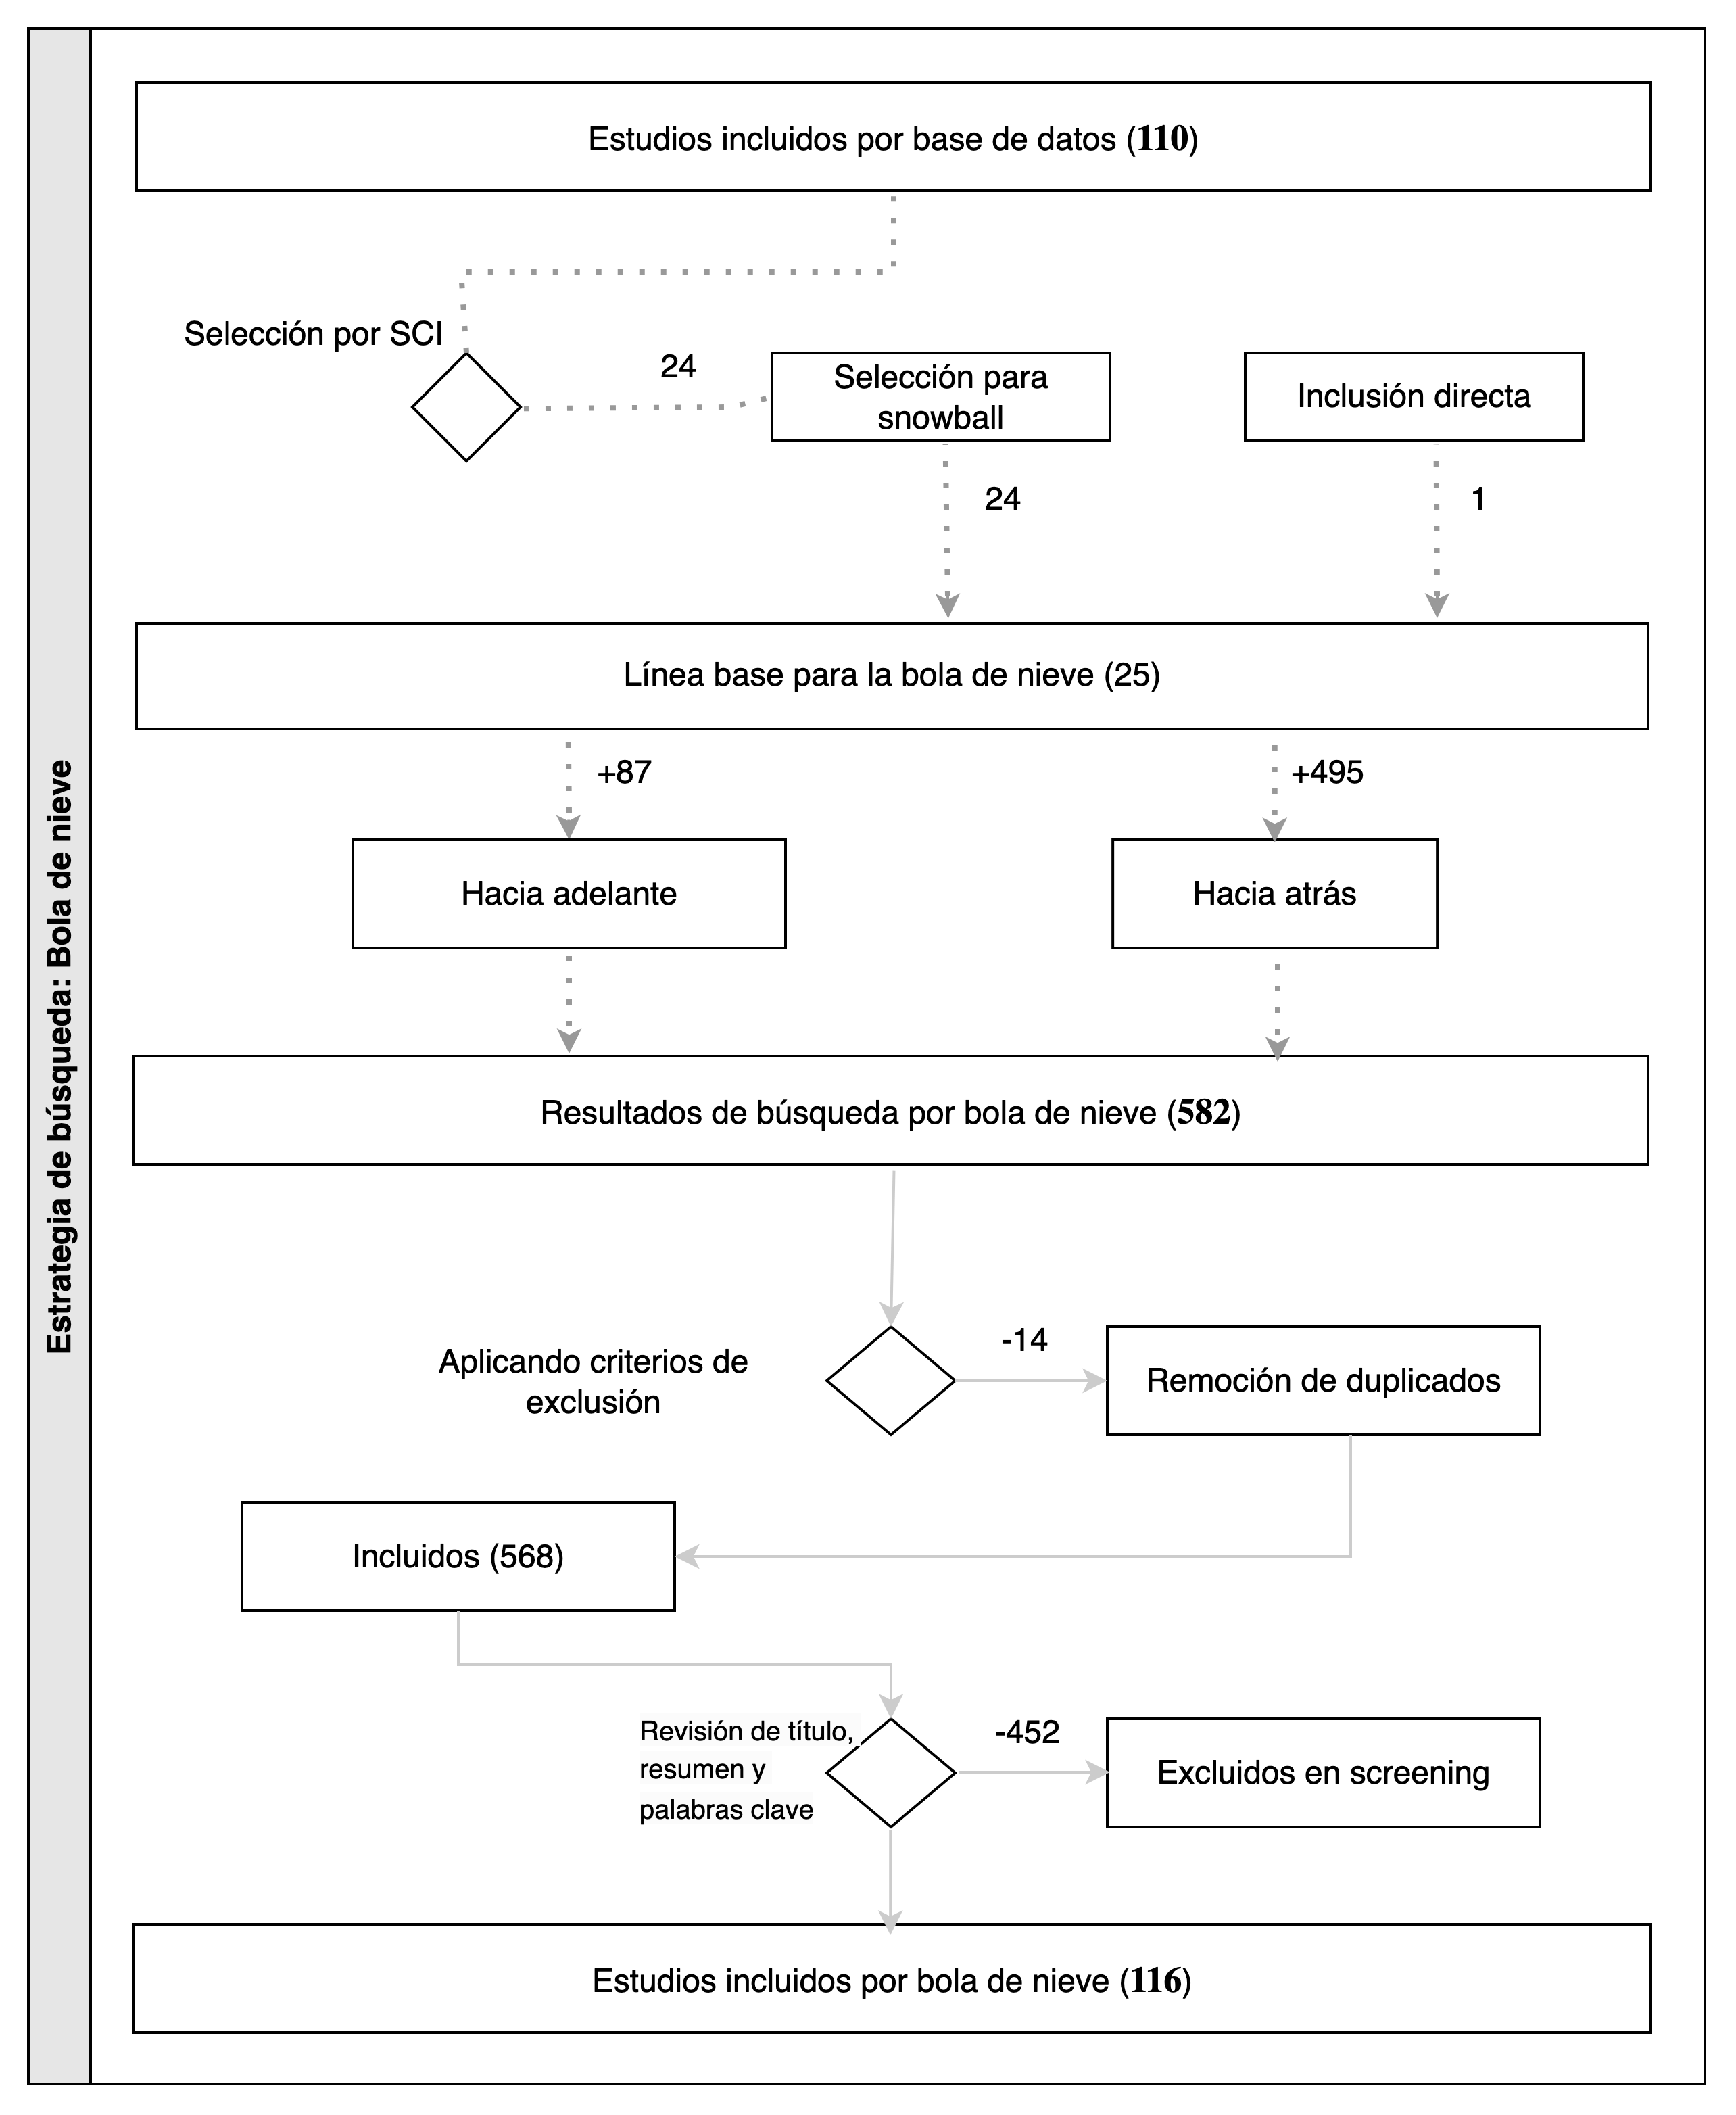
\includegraphics[scale=0.14]{tablas-images/cp2/diagrama-bola-nieve-busqueda.png}
    \caption{Diagrama de la búsqueda en bola de nieve}\label{tab:tabla-diagrama-bola-nieve-busqueda}
\end{table}

\section{Identificación de estudios}

\subsection{Artículos por año y métricas}
\noindent
A continuación se presentan las gráficas de los resultados de la búsqueda.
En la figura~\ref{fig:diagrama-articulos-ano-metrica} se pueden visualizar las métricas de calidad, separadas por los últimos 3 años y mostrando el promedio en cada métrica de los artículos publicados en esos años, así como un apartado donde se calcula la sumatoria de estas métricas por cada año.

\begin{figure}[H]
    \centering
    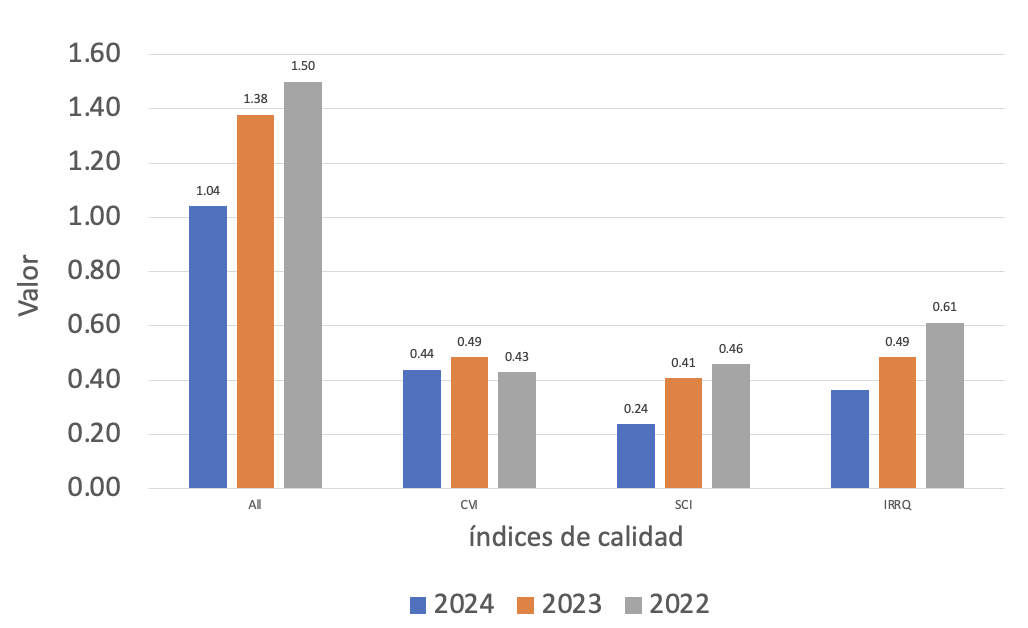
\includegraphics[scale=0.7]{tablas-images/cp2/diagrama-articulos-ano-metrica.png}
    \caption{Artículos por métricas y año}\label{fig:diagrama-articulos-ano-metrica}
\end{figure}

En la figura~\ref{fig:tipos-articulos} se muestra el conteo de artículos por su tipo específico, el cual puede ser uno de 3 opciones: 'Revista', 'Conferencia' o 'Genérico'. Vemos que la mayoría de artículos provienen de revistas.
\begin{figure}[H]
    \centering
    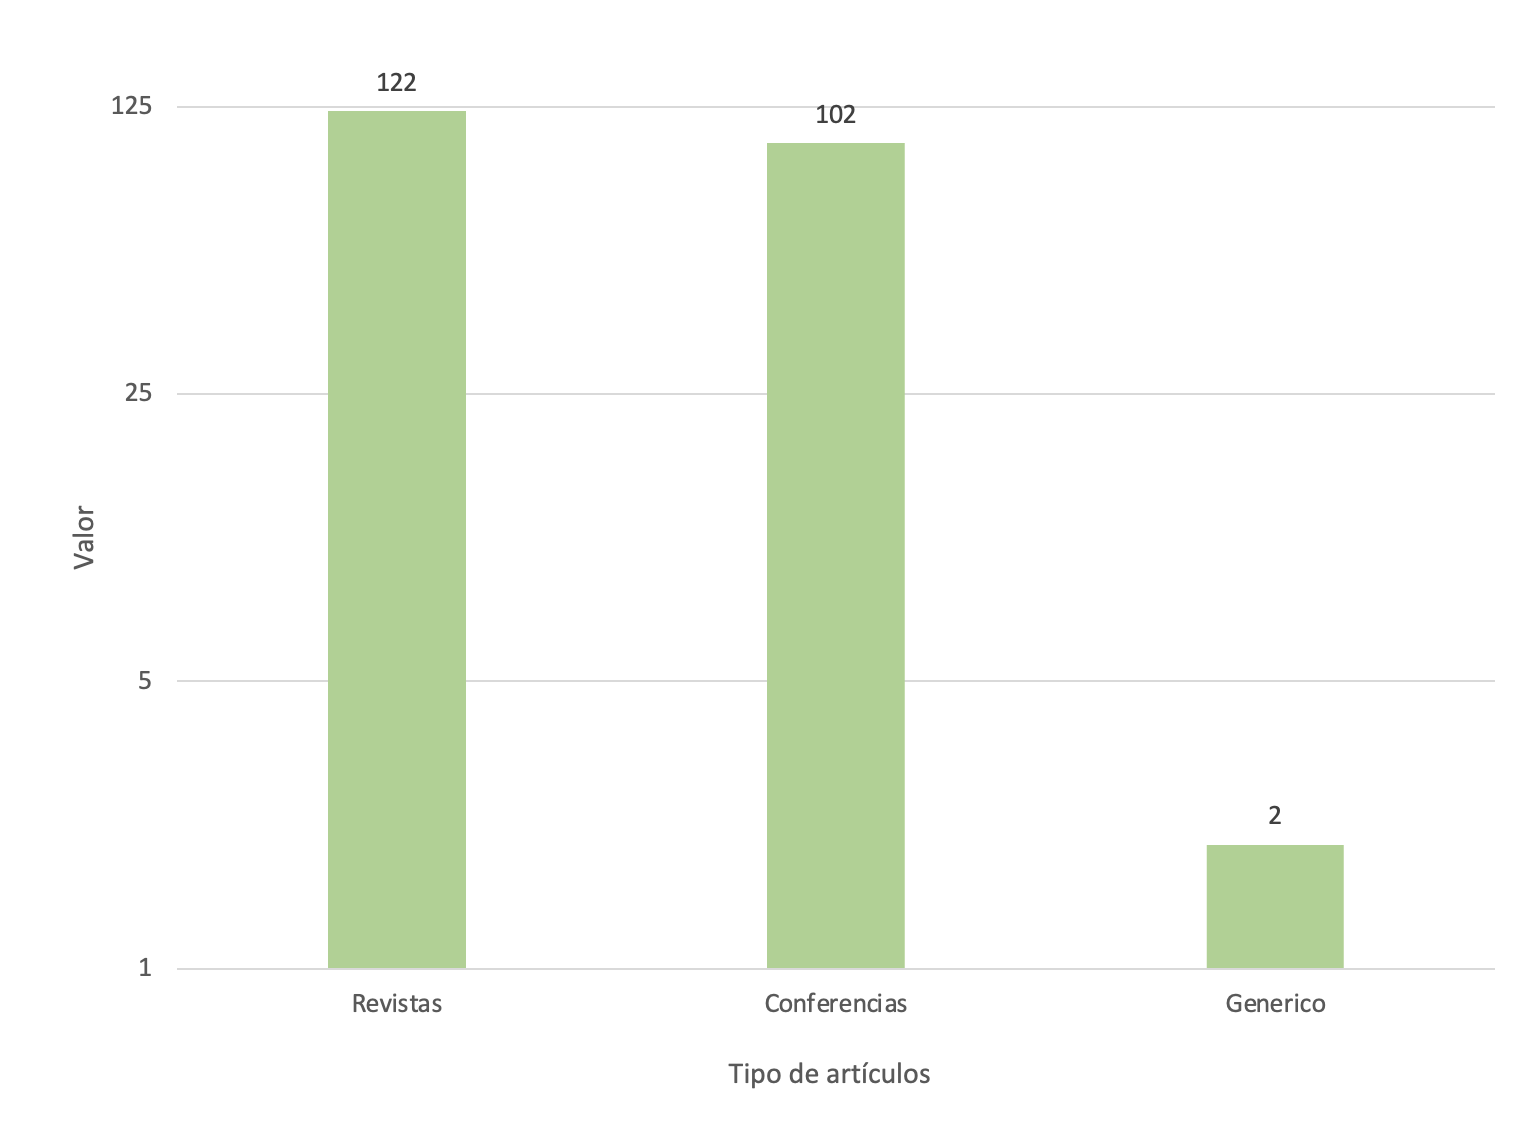
\includegraphics[scale=0.5]{tablas-images/cp2/tipos-articulos.png}
    \caption{Artículos por tipo}\label{fig:tipos-articulos}
\end{figure}

En la figura~\ref{fig:estrategia-busqueda-articulos} se detalla la cantidad de artículos que se extrajeron de cada estrategia. Se puede observar que la estrategia que generó más artículos fue la técnica de ~\textit{Snowball}.
\begin{figure}[H]
    \centering
    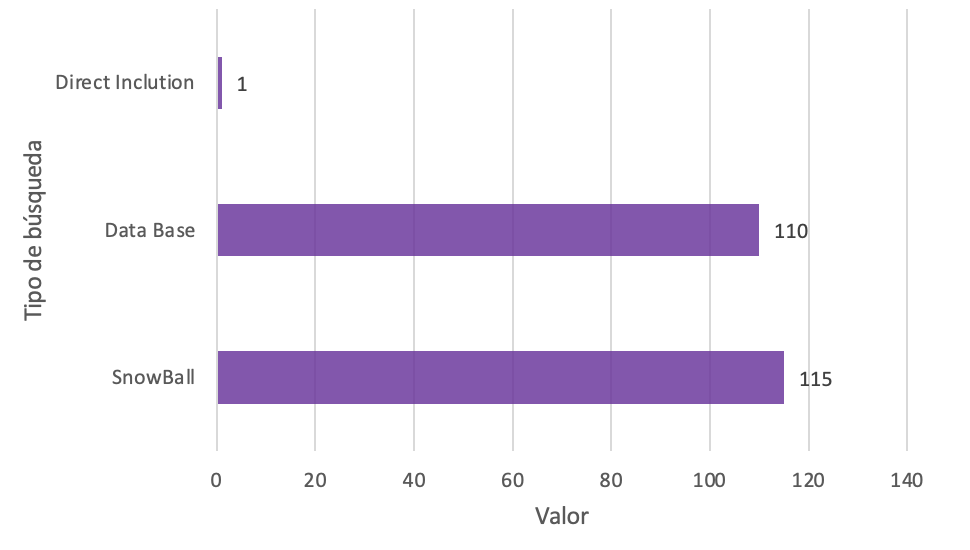
\includegraphics[scale=0.8]{tablas-images/cp2/estrategia-busqueda-articulos.png}
    \caption{Estrategia de búsqueda de artículos}\label{fig:estrategia-busqueda-articulos}
\end{figure}

Finalmente, en la figura~\ref{fig:diagrama-red-articulos} se puede apreciar un diagrama de red, que segrega por colores los tópicos más relacionados entre sí, vemos 4 grandes grupos: IA, cloud computing, virtualización, desarrollo de software.
\begin{figure}[H]
    \centering
    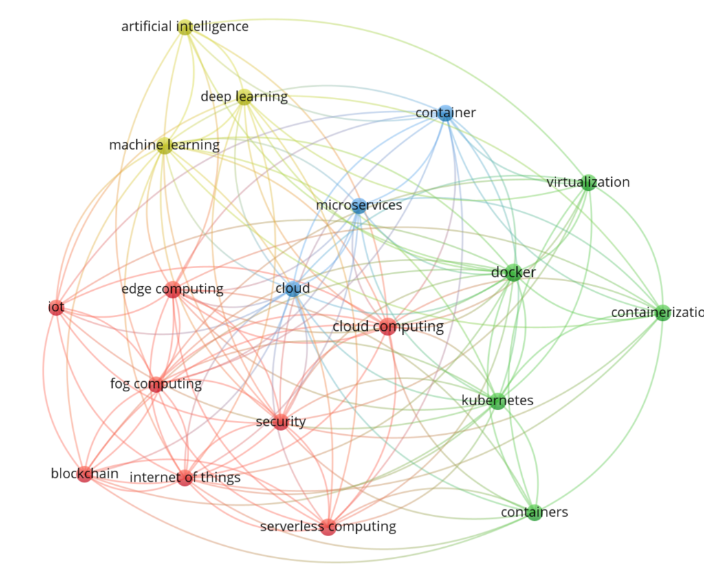
\includegraphics[scale=0.9]{tablas-images/cp2/diagrama-red-busqueda.png}
    \caption{Diagrama de red de los artículos}\label{fig:diagrama-red-articulos}
\end{figure}

\section{Identificación de tecnologías de \VBC}\label{sec:tecnologias-vbc-identificadas}
\noindent
En esta sección se presentan las tecnologías de \VBC\ y las tecnologías de orquestación identificadas en el proceso de revisión sistemática de la literatura. \\
\noindent
El gráfico presentado en la Figura XXXXXX expone la distribución de las tecnologías de \VBC\ identificadas en el estudio de mapeo sistemático. En él se observa que Docker es la tecnología con mayor representación, acumulando 94 menciones, lo que evidencia su posición dominante en el ecosistema. En contraste, alternativas como Podman, LXC y Containerd muestran una presencia moderada, mientras que tecnologías como OpenVZ y Hyper-V containers apenas alcanzan una mención. Este comportamiento refleja tanto la consolidación de Docker como estándar \textit{de facto} en el ámbito de los contenedores, como la coexistencia de múltiples soluciones que, aunque menos extendidas, representan enfoques relevantes para casos de uso específicos. \\
\input{tablas-images/cp2/tecnologias-vbc.tex}
\noindent
La Figura XXXXXX muestra la distribución de las tecnologías de orquestación identificadas en el estudio de mapeo sistemático. El gráfico evidencia una clara predominancia de Kubernetes, con 67 menciones, consolidándose como la solución de referencia en la gestión de contenedores. En un segundo nivel, tecnologías como Docker Swarm (9) y Apache Mesos (5) presentan una adopción moderada, mientras que opciones como OpenShift, Docker Compose, Amazon ECS y Amazon EKS aparecen con una menor representación. Estos resultados reflejan la consolidación de Kubernetes como estándar en orquestación, a la vez que destacan la diversidad de alternativas que, aunque menos extendidas, atienden necesidades específicas en determinados contextos.
\input{tablas-images/cp2/tecnologias-orquestacion.tex}

\section{Información de la herramienta}

\noindent
La herramienta utilizada para este proceso de revisión de la literatura fue \textbf{SMS-BUILDER}, la cual se encuentra disponible en \textit{Docker Hub}. La imagen puede consultarse en el siguiente enlace:

\begin{center}
	\href{https://hub.docker.com/r/griduq/sms-builder}{\texttt{https://hub.docker.com/r/griduq/sms-builder}}
\end{center}



\section{Reproducibilidad del método}
\noindent
Con el fin de fomentar la reproducibilidad del método de revisión, se proporcionan dos mecanismos de verificación que permiten a los revisores y lectores acceder de forma transparente a la información utilizada, generada mediante la herramienta SMS-Builder de~\cite{SMSBuilder2020}
\begin{itemize}
	\item Un enlace de acceso público a la instancia de SMS-Builder que contiene todos los datos del proceso de revisión sistemática: \href{https://sms-vbc.iti.grid.uniquindio.edu.co/sms.xhtml}{link}. Las credenciales de acceso son ``invitado'' tanto para el nombre de usuario como para la contraseña.
	\item Una imagen de Docker de acceso público que integra toda la documentación necesaria para crear un contenedor con los datos del proceso: \href{https://hub.docker.com/r/anubis1001/tg-vbc-sms-builder}{link}.
\end{itemize}

\noindent
Adicionalmente, se implementaron procesos de respaldo como medida de seguridad. Estos \textit{backups} fueron almacenados en ubicaciones diferentes, siguiendo la estrategia de respaldo \textbf{3--2--1}.

\section{Conclusiones de la revisión sistemática de la literatura}
\noindent
Esta sección presenta un mapeo sistemático de la literatura sobre tecnologías de virtualización basadas en contenedores, principalmente relacionada con la educación, la investigación y la extensión. Dentro del \SMS, se definió un esquema de clasificación según los temas específicos establecidos durante la fase de planificación. Este esquema proporciona un mapeo de la información en tablas y gráficos estadísticos que ayudan a describir los datos y su relación con las preguntas de investigación. El mapeo sistemático reveló una creciente proliferación de estudios relacionados con las tecnologías de \VBC, incluyendo estudios en diferentes áreas y aplicaciones. Esta proliferación de estudios podría ser contraproducente para ciertas partes interesadas a la hora de implementar arquitecturas con estas tecnologías. Además, puede provocar una saturación de la literatura y dificultar el desarrollo, principalmente debido al abrumador volumen de información disponible. Más allá de los resultados obtenidos en este \SMS, los estudios se analizaron explorando la información subyacente y las tendencias. De este modo, se identificó una creciente adopción de la virtualización ligera en la implementación de soluciones, con especial énfasis en la computación en la nube y orquestadores como Kubernetes. Este liderazgo se ve reforzado por la necesidad de las organizaciones de proporcionar redundancia, fiabilidad y escalabilidad en sus aplicaciones y servicios.
